% !TEX root = deckblatt4.tex
\section{Messung eines Rechtecksignals}
\subsection{Aufgabenstellung}
Hier sollte ein Rechtecksignal in Zeit und Frequnenzbereich gemessen werden und anschlie\ss{}end die Ergebnisse erl\"autert werden

\subsection{Vorbereitung \& Messaufbau}
Es wurde mit dem Frequnezgenerator ein Rechtecksingal mit einer Amplitude von $1V_{pp}$ und einer Frequnez von $10kHz$ erzeugt. Der Ausgang des Frequnezgenerators wurde direkt mit dem Tastkopf des Oszilloskops verbunden, es wurde keine Messschaltung aufgebaud.

\begin{figure}[H]
 \begin{center}
  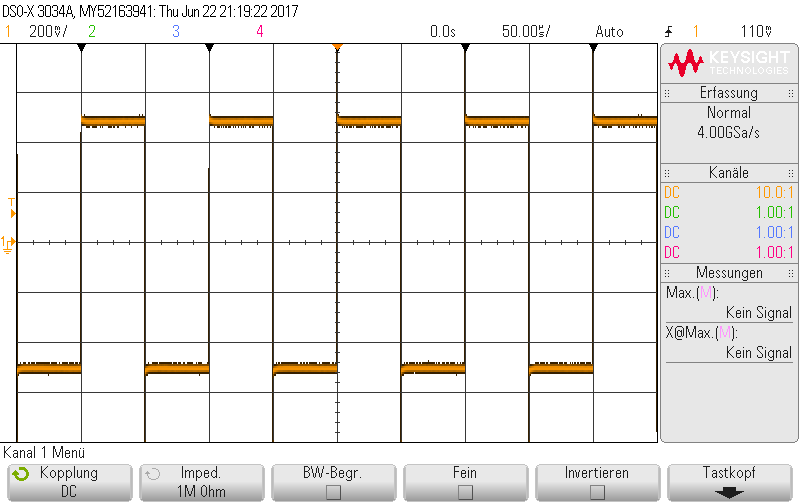
\includegraphics[height=6cm,width=12cm]{OsziBilder/bsp2_time.png}
 \end{center}
 \caption{Rechteckspannung $1V_{pp}$, $10kHz$}\label{bsp2_time}
\end{figure}
\noindent
In Abbildung \ref{bsp2_time} ist, dass Rechtecksignal, welches zur Messung verwendet wurde im Zeitbereich zu sehen. \\
\newpage

\subsection{FFT}
In dieser Messung wurde das Hanning-Fenster verwendet, da dies ein sehr einfaches und g\"angiges Fenster ist.

\begin{figure}[H]
 \begin{center}
  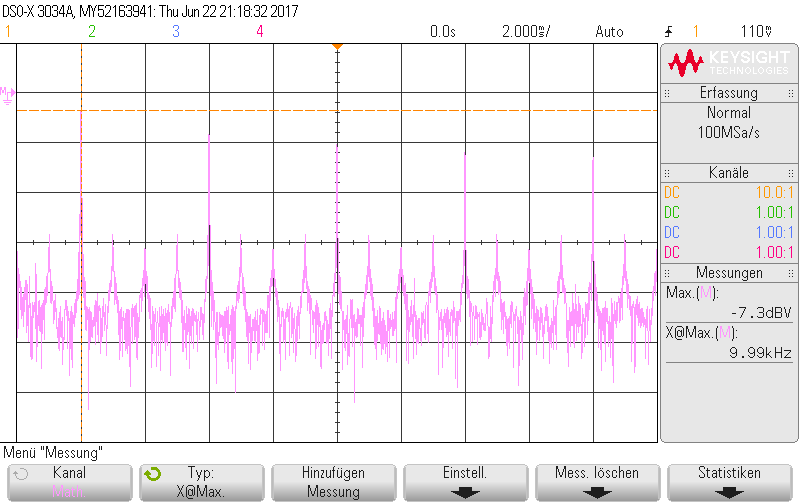
\includegraphics[height=6cm,width=12cm]{OsziBilder/bsp2_Hanning_dB.png}
 \end{center}
 \caption{Rechteckspannung $1V_{pp}$, $10kHz$}\label{bsp2_dB}
\end{figure}
\noindent

\begin{figure}[H]
 \begin{center}
  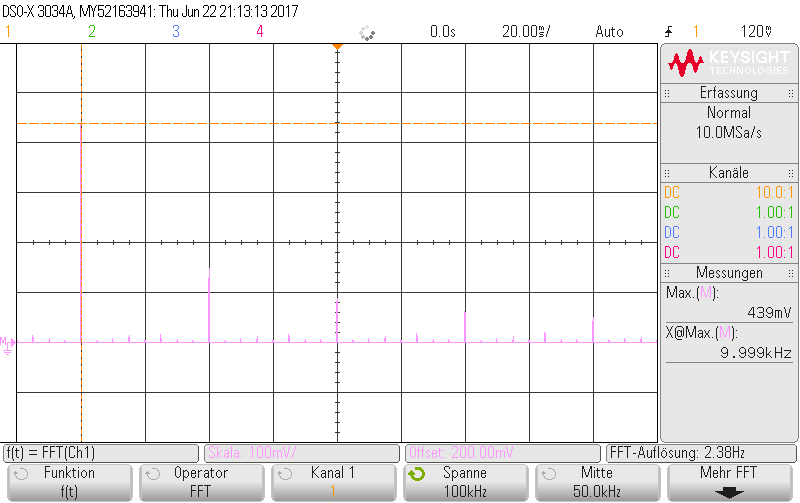
\includegraphics[height=6cm,width=12cm]{OsziBilder/bsp2_Hanning_RMS_Cursor.png}
 \end{center}
 \caption{Rechteckspannung $1V_{pp}$, $10kHz$}\label{bsp2_rms}
\end{figure}
\noindent
In den beiden Abbildungen \ref{bsp2_dB} \& \ref{bsp2_rms} sind die Spektren des oben gezeigten Rechecksignals zu sehen. In Abbildung \ref{bsp2_dB} wurde f\"ur die y-Achse eiene Logarithmische dB Skalierung verwendet und in Abbildung \ref{bsp2_rms} eine lineare. \\
In den Beiden Abbildungen ist der der Vorteil der dB - Skalierung deutlich zu erknnen. W\"ahrend in Abbildung \ref{bsp2_dB} die Amplitude bei $90kHz$ nur um etwar $10dB$ kleiner als die der Grundfrequnez, so ist diese in der Linearen Darstellung schon verschwindend gering. \newpage \noindent
Wie erwartet stechen bei einem Symetrischen Rechteck alle Ungeraden Vielfachen der Grundfrequnez hervor. Warum dies so ist l\"asst sich mathematisch leicht begr\"unden \\ \\
Eine Rechteckfunktion ist folgenderma\ss{}en definiert:
\begin{center}
    $f(t) = \left\{\begin{array}{ll}
            1        \hspace{1.5cm} 0\leq t < \pi\\
            0        \hspace{1.5cm} \pi \leq t < 2\pi
            \end{array}\right.$
\end{center}
\noindent
Diese Funktion ist Rotationssymetrisch und somit sind alle cos-Anteile 0
\begin{center}
  \begin{align*}
    a_0 &= \frac{1}{2\pi}\int_0^{\pi} 1 dt = \frac{1}{2} \\
    b_n &= \frac{1}{2\pi}\int_0^{\pi} sin(nt) dt \\
    b_n &= \frac{1}{2\pi} \\
    b_n &= \frac{1}{2\pi} \left[ -\frac{cos(n\pi)}{n} + \frac{1}{n} \right] = -\frac{1}{2n\pi} \left[ (-1)^n - 1  \right] \\
    b_n &= \left\{\begin{array}{ll}
            0              \hspace{1.5cm} \text{f\"ur n gerade}\\
            \frac{1}{n\pi} \hspace{1.3cm} \text{f\"ur n ungerade}
            \end{array}\right. \\
  \end{align*}
\end{center}
\noindent
Am Ergebnis der Fourierreihe ist zu sehen, dass die Spektralanteile f\"ur alle geraden Vielfachen der Grundfrequnez 0 Eregeben, und die Amplituden der ungeraden Anteile mit dem Faktor $\frac{1}{n\pi}$ kleiner werden.

\begin{figure}[H]
  \begin{center}
    \begin{tabular}{|c|c|} \hline
    $f_g=10kHz$ & $439mV$ \\ \hline
    $3*f_g$ & $147,11mV$ \\ \hline
    $5*f_g$ & $90,77mV$ \\ \hline
    $7*f_g$ & $62,60mV$ \\ \hline
    \end{tabular}
  \end{center}
  \caption{Messwerte der Hauptkomponente und der ersten 3 Nebenkomponenten}
\end{figure}
\noindent
In obiger Tabelle sind die Amplitden zu der Grundrequnez und den ersten drei ungeraden Vielfachen herausgemessen worden. Man kann sehr gut erkennen, dass die Werte exponentiell kleiner werden.
